\documentclass[12pt,a4paper]{report}

\usepackage[left=3.0cm,right=2.25cm,top=2.5cm,bottom=2.4cm,headheight=15pt]{geometry}
\usepackage{mathptmx}
\usepackage[T1]{fontenc}
\usepackage{amsmath,amssymb}
\usepackage{setspace}
\usepackage{graphicx}
\usepackage{booktabs,array}
\usepackage{enumitem}
\usepackage{fancyhdr}
\usepackage{titlesec}
\usepackage{tikz}
\usetikzlibrary{arrows.meta,positioning,shapes.geometric,calc}
\usepackage[hidelinks]{hyperref}
\usepackage{caption}
\usepackage{tocloft}

% =====================================================================
%  GCOERC NASHIK - T.E. COMPUTER ENGINEERING SEMINAR REPORT TEMPLATE
%  Content filled from pooja-report.docx.
%  Keep logo.jpg (college) and sppu.jpg (university) in the same folder.
%  Compile with:  pdflatex report.tex  (run twice)  or  latexmk -pdf report.tex
% =====================================================================
\newcommand{\ttitle}{Agentic AI Systems: Architecture and Evaluation Using a Frictionless Parking Scenario}
\newcommand{\TTITLE}{AGENTIC AI SYSTEMS: ARCHITECTURE AND EVALUATION USING A FRICTIONLESS PARKING SCENARIO}
\newcommand{\studentname}{Pooja Laxman Makone}
\newcommand{\rollno}{203}
\newcommand{\guidename}{Mrs.\ Pradnya Bachhav}
\newcommand{\acadyear}{2026--27}

\captionsetup{font=small,labelfont=bf}
\setlength{\parindent}{1.2em}
\setlength{\parskip}{0pt}

% ---------- chapter / section styling (as in college template) ----------
\titleformat{\chapter}[display]
  {\normalfont\bfseries\centering}{\large Chapter \thechapter}{10pt}{\large\uppercase}
\titlespacing*{\chapter}{0pt}{0pt}{16pt}
\titleformat{\section}{\normalfont\large\bfseries}{\thesection}{0.8em}{}
\titleformat{\subsection}{\normalfont\normalsize\bfseries}{\thesubsection}{0.8em}{}
\titlespacing*{\section}{0pt}{10pt}{4pt}
\titlespacing*{\subsection}{0pt}{8pt}{3pt}

% ---------- header / footer ----------

\fancypagestyle{main}{%
  \fancyhf{}
  \fancyhead[C]{\scriptsize \ttitle}
  \fancyfoot[C]{\small\thepage\\[1pt]\scriptsize Department of Computer Engineering, GCOERC, Nashik 2026--27}
  \renewcommand{\headrulewidth}{0.4pt}
  \renewcommand{\footrulewidth}{0pt}}
\pagestyle{main}
\fancypagestyle{plain}{\fancyhf{}%
  \fancyhead[C]{\scriptsize \ttitle}
  \fancyfoot[C]{\small\thepage\\[1pt]\scriptsize Department of Computer Engineering, GCOERC, Nashik 2026--27}
  \renewcommand{\headrulewidth}{0.4pt}}

\newcommand{\unnumchapter}[1]{%
  \chapter*{#1}\addcontentsline{toc}{chapter}{#1}}

% ---------- page border for cover and certificates ----------
\newcommand{\pageborder}{%
\begin{tikzpicture}[remember picture,overlay]
\draw[line width=1.6pt] ($(current page.north west)+(1.5cm,-1.5cm)$) rectangle ($(current page.south east)+(-1.5cm,1.5cm)$);
\end{tikzpicture}}

% ---------- TOC look: chapters bold, sections indented ----------
\renewcommand{\cftchapfont}{\bfseries\small}
\renewcommand{\cftchappagefont}{\bfseries\small}
\renewcommand{\cftsecfont}{\small}
\renewcommand{\cftsecpagefont}{\small}
\renewcommand{\cftsubsecfont}{\small}
\renewcommand{\cftsubsecpagefont}{\small}
\setlength{\cftbeforechapskip}{6pt}
\setlength{\cftbeforesecskip}{1pt}
\setcounter{tocdepth}{2}
\renewcommand{\cfttoctitlefont}{\hfill\normalfont\large\bfseries}
\renewcommand{\cftaftertoctitle}{\hfill}
\renewcommand{\cftloftitlefont}{\hfill\normalfont\large\bfseries}
\renewcommand{\cftafterloftitle}{\hfill}
\setlength{\cftbeforetoctitleskip}{0pt}
\setlength{\cftbeforeloftitleskip}{0pt}
\renewcommand{\cftchapdotsep}{\cftdotsep}
\renewcommand{\cftfigfont}{\small}
\renewcommand{\cftfigpagefont}{\small}

\begin{document}

% ------------------------------ COVER ------------------------------
\begin{titlepage}
\thispagestyle{empty}
\pageborder
\centering
\singlespacing
\vspace*{0.3cm}
{\large\bfseries A\par}\vspace{6pt}
{\large\bfseries SEMINAR REPORT\par}\vspace{6pt}
{\large\bfseries ON\par}\vspace{10pt}
{\Large\bfseries \TTITLE\par}
\vspace{14pt}
{\normalsize SUBMITTED TO THE SAVITRIBAI PHULE PUNE UNIVERSITY IN FULFILMENT OF THE REQUIREMENTS\\ FOR THE AWARD OF THE\par}
\vspace{8pt}
{\large\bfseries THIRD YEAR COMPUTER ENGINEERING\par}\vspace{8pt}
{\large\bfseries BY\par}
{\large\bfseries \studentname\par}
{\normalsize (Roll No: \rollno)\par}\vspace{8pt}
{\large\bfseries UNDER THE GUIDANCE OF\par}
{\large\bfseries \guidename\par}\vspace{10pt}

\includegraphics[height=3.6cm]{logo.jpg}\par\vspace{10pt}
{\normalsize\bfseries DEPARTMENT OF COMPUTER ENGINEERING\\
Guru Gobind Singh College of Engineering and Research Center, Nashik.\\
Khalsa Educational Complex, Guru Gobind Singh Marg, Wadala--Pathardi Road, Indira Nagar, Nashik, Maharashtra 422009\\
YEAR \acadyear\par}
\end{titlepage}

% --------------------------- CERTIFICATE 1 -------------------------
\thispagestyle{empty}
\pageborder
\begin{center}
\singlespacing
\vspace*{0.4cm}
{\normalsize\bfseries DEPARTMENT OF COMPUTER ENGINEERING\\
Guru Gobind Singh College of Engineering and Research Center, Nashik\\
Khalsa Educational Complex, Guru Gobind Singh Marg, Wadala--Pathardi Road, Indira Nagar, Nashik, Maharashtra 422009\\
Year \acadyear\par}
\vspace{10pt}

\includegraphics[height=3.4cm]{logo.jpg}\\[14pt]
{\large\bfseries CERTIFICATE}\\[8pt]
{\bfseries This is to certify that seminar report entitled}\\[10pt]
{\large\bfseries ``\TTITLE''}\\[10pt]
is submitted as fulfilment of curriculum of the T.E.\ Computer Engineering\\[10pt]
{\bfseries BY}\\[8pt]
{\bfseries \studentname}\\
{\bfseries (Roll No: \rollno)}
\end{center}
\vspace{40pt}
\begin{center}
\singlespacing\small
\begin{tabular}{p{0.28\textwidth}p{0.36\textwidth}p{0.24\textwidth}}
\guidename & Dr.\ Swati Khokale \& Mr.\ Ajit Pagar & Dr.\ Nita Thakare\\
\textbf{Seminar Guide} & \textbf{Seminar Coordinator} & \textbf{Head of Dept.}
\end{tabular}
\end{center}
\vfill
{\singlespacing\noindent\hspace{0.6cm}\textbf{Place:} GCOERC, Nashik\\
\hspace*{0.6cm}\textbf{Date:}\par}
\vspace{1.4cm}
\clearpage

% --------------------------- CERTIFICATE 2 -------------------------
\thispagestyle{empty}
\pageborder
\begin{center}
\singlespacing
\vspace*{0.4cm}
{\normalsize Savitribai Phule Pune University\par}\vspace{6pt}

\includegraphics[height=3.4cm]{sppu.jpg}\\[12pt]
{\large\bfseries CERTIFICATE}\\[10pt]
This is to certify that\\[8pt]
{\bfseries \studentname}\\
{\bfseries (Roll No: \rollno)}\\[10pt]
Student of T.E.\ Computer\\[4pt]
Was examined in Seminar Report entitled\\[10pt]
{\large\bfseries ``\TTITLE''}\\[12pt]
on \underline{\hspace{0.8cm}} / \underline{\hspace{0.8cm}} /2026\\[8pt]
At\\[4pt]
DEPARTMENT OF COMPUTER ENGINEERING,\\
GURU GOBIND SINGH COLLEGE OF ENGINEERING AND RESEARCH CENTER, NASHIK\\[4pt]
{\bfseries YEAR \acadyear}
\end{center}
\vspace{50pt}
\begin{center}
\begin{tabular}{p{0.38\textwidth}p{0.38\textwidth}}
\dotfill & \dotfill\\
\centering Internal Examiner & \centering External Examiner\tabularnewline
\end{tabular}
\end{center}
\clearpage

\pagenumbering{roman}
\setcounter{page}{1}
\onehalfspacing

% ------------------------------ ABSTRACT ---------------------------
\unnumchapter{ABSTRACT}
Agentic Artificial Intelligence (AI) is an emerging technology that enables AI systems to understand goals, make decisions, and perform tasks with limited human intervention. Unlike traditional AI systems that mainly respond to user inputs, agentic AI systems can use memory, tools, and reasoning to complete complex tasks. This seminar presents the architecture and evaluation of agentic AI systems using a frictionless parking scenario.

The proposed architecture consists of seven specialized agents: Interaction Agent, Informative Search Agent, On-Route Guidance Agent, Access Agent, Micro-Routing Agent, On-Spot Agent, and Departure Agent. These agents are designed to cooperate to provide a smooth parking experience, from understanding the user's requirements to assisting with parking and departure. The architecture also includes foundation models, prompt templates, short-term and long-term memory, and external tools.

The research evaluates the Interaction Agent and Informative Search Agent by examining response latency and lexical consistency under different experimental conditions. The results highlight the importance of model selection, prompt specificity, query complexity, and response verbosity in agent performance. The study demonstrates the potential of agentic AI for coordinating complex, multi-step tasks while also identifying challenges related to response consistency and system performance.

\vspace{6pt}
\noindent\textbf{\emph{Keywords---Agentic AI; Autonomous Agents; Large Language Models (LLMs); Multi-Agent Systems; Memory; Tool Use; Frictionless Parking.}}
\clearpage

% -------------------------- ACKNOWLEDGEMENT ------------------------
\unnumchapter{ACKNOWLEDGEMENT}
It is my immense pleasure to work on this seminar \textbf{\ttitle}. It is only the blessing of my divine master which has prompted and mentally equipped me to undergo the study of this seminar.

I would like to thank \textbf{Prof.\ (Dr.) N.\ G.\ Nikam}, Principal, Guru Gobind Singh College of Engineering and Research Center, for giving me such an opportunity to develop practical knowledge about the subject. I am also thankful to \textbf{Dr.\ Nita M.\ Thakare}, Head of Computer Engineering Department, for her valuable encouragement at every phase of my seminar work and completion.

I offer my sincere thanks to my guide \textbf{\guidename}, who very affectionately encouraged me to work on the subject and gave valuable guidance from time to time. While preparing this seminar I am very much thankful to her.

I am also grateful to the entire staff of Computer Engineering Department for their kind co-operation, which helped me in the successful completion of this seminar.

\vspace{30pt}
\hfill\begin{minipage}{0.45\textwidth}
\singlespacing
\textbf{\studentname}\\
\textbf{Roll No: \rollno}\\[6pt]
GCOERC, NASHIK.
\end{minipage}
\clearpage

% ------------------------------- INDEX -----------------------------
\begingroup
\singlespacing
\renewcommand{\contentsname}{INDEX}
\addcontentsline{toc}{chapter}{INDEX}
\tableofcontents
\clearpage
\renewcommand{\listfigurename}{LIST OF FIGURES}
\addcontentsline{toc}{chapter}{LIST OF FIGURES}
\listoffigures
\endgroup
\clearpage

\pagenumbering{arabic}
\setcounter{page}{1}
\onehalfspacing

% ----------------------------- CHAPTER 1 ---------------------------
\chapter{INTRODUCTION}
Artificial Intelligence (AI) is a growing technology that allows computer-based systems to accomplish functions typically performed by humans, including speech understanding, problem-solving, decision-making, etc. Due to advancements in the field of Large Language Models (LLMs) and Large Reasoning Models (LRMs), AI systems become increasingly capable of accomplishing complicated tasks. The Agentic Artificial Intelligence (Agentic AI) is a new technological concept, which assumes the functioning of artificial intelligence systems based on reasoning, memory, and using external means in pursuit of certain objectives. Contrary to conventional AI systems that only respond to questions posed by users, agentic AI systems are able to plan their actions, use available means and interact with other agents.

The research paper, ``Agentic AI Systems: Architecture and Evaluation using a Frictionless Parking Scenario,'' by Alaa Khamis~\cite{ref1} provides a model for analyzing the working of agentic AI systems in a practical environment. The study proposes a frictionless parking scenario wherein there will be multiple specialized agents for helping the user with his parking needs. There are seven agents involved in the architecture: Interaction Agent, Informative Search Agent, On-Route Guidance Agent, Access Agent, Micro-Routing Agent, On-Spot Agent, and Departure Agent. All of these agents are assigned particular responsibilities in order to ensure smooth functioning.

The research also evaluates the implemented Interaction Agent and Informative Search Agent using performance metrics such as response latency and lexical consistency. The study examines how factors such as model selection, prompt specificity, query complexity, and response verbosity affect agent performance. This seminar focuses on understanding the basic concepts of Agentic AI, its architecture, the coordination of specialized agents, and the evaluation of their performance using the frictionless parking scenario.

\section{Motivation}
Motivation behind investigating Agentic AI comes from the desire to learn about how AI systems can not only answer questions individually but also assist in completing complex tasks by executing actions.

Main motivations for investigation include:
\begin{itemize}[leftmargin=*]
  \item \textbf{Task automation:} Agentic AI can break down the complex task into smaller actions and execute them using specialized agents.
  \item \textbf{Enhancement of user experience:} Contextual and personalized aid offered by AI agents according to the needs of users.
  \item \textbf{Agents' coordination:} Coordination among agents working towards achieving a common goal.
  \item \textbf{Agents' use of memory and external tools:} Agents can employ information available in their memory or use external tools to accomplish actions.
  \item \textbf{Latency and lexical consistency:} Evaluation of performance of the system is done with respect to latency and lexical consistency. Frictionless Parking is an instance of applying the above concepts in practice.
\end{itemize}

\section{Problem Statement}
Conventional digital assistants tend to provide aid in handling isolated queries or task-related prompts. On the other hand, some complex real-life activities could involve multiple interconnected actions, continuous exchange of information, and cooperation between various functionalities.

For instance, in the context of parking, the user may require help in obtaining parking-related information, navigation to the destination, gaining access to the parking facility, parking, and exiting from the parking site. Handling each action separately and independently would result in a less convenient interaction with the user.

To solve this problem, the research introduces an example of an agentic AI system where multiple agents with various functionalities are supposed to collaborate during the parking process. Moreover, the impact of model configurations and prompt parameters on the agents' response latency and lexical consistency is being investigated.

Thus, the major issue is the development and evaluation of a collaborative agentic AI system.

% ----------------------------- CHAPTER 2 ---------------------------
\chapter{OBJECTIVES}
The main objectives of this seminar are:
\begin{enumerate}[leftmargin=*]
  \item To understand the fundamental concepts and working principles of Agentic Artificial Intelligence (AI).
  \item To study the architecture of an agentic AI system using the frictionless parking scenario.
  \item To understand the roles and functions of the seven specialized agents involved in the proposed architecture.
  \item To study how AI agents coordinate and cooperate using different interaction and cooperation patterns.
  \item To understand the role of foundation models, prompt templates, memory systems, and tools in agentic AI.
  \item To identify the potential applications, advantages, limitations, and future scope of agentic AI systems.
\end{enumerate}

% ----------------------------- CHAPTER 3 ---------------------------
\chapter{LITERATURE REVIEW}
The literature relevant to this seminar can be grouped into four themes: the conceptual foundations of agentic AI, the architectures and enabling components that realise it, multi-agent coordination and communication, and the evaluation of agentic systems. This section reviews the available sources along these themes and identifies the gaps that motivate the study of an agentic AI system for frictionless parking.

\noindent\textbf{Conceptual foundations and agency.}
Acharya et al.~\cite{ref2} present agentic AI as a paradigm in which autonomous systems pursue complex, long-horizon goals with minimal human supervision, distinguishing it from classical rule-based AI and from generative AI through its autonomy, goal-orientation and adaptability. They argue that the development of such systems rests on reinforcement learning, goal-oriented architectures and adaptive control, and that these foundations allow an agent to revise its strategy as conditions change. Complementing this capability-focused view, Miehling et al.~\cite{ref7} contend that the field is overly focused on individual model capability and that a systems-theoretic perspective is required to understand the behaviour of an agentic system as a whole. They formalise \emph{functional agency} through three conditions---action generation, an outcome model, and adaptation---and argue that the collective agency of a system can emerge from the interaction of comparatively simple agents with one another, with humans and with the environment, rather than from the capability of any single component. Their analysis also highlights two persistent weaknesses of current LLM-based agents, namely limited causal reasoning and a lack of metacognitive awareness, which they treat as open challenges rather than solved problems.

\noindent\textbf{Architectures, memory and tool use.}
Derouiche et al.~\cite{ref8} provide a systematic comparison of leading agentic AI frameworks, including CrewAI, LangGraph, AutoGen, Semantic Kernel, Agno, Google ADK and MetaGPT, and evaluate them along architectural principles, communication mechanisms, memory management, safety guardrails and service-oriented alignment. Their comparison shows that these frameworks, despite different design priorities, share a common set of components: a foundation model for reasoning, external tools for action, memory for context, and guardrails for safety and validation. They further show that the memory support offered by frameworks varies considerably, with some providing only short-term, session-level state while others support long-term, semantic, procedural and episodic memory. The survey of Acharya et al.~\cite{ref2} reaches a similar conclusion, identifying tool use and memory mechanisms---in particular episodic and semantic memory---as core capabilities that allow an agent to retain context and improve its decisions over time.

\noindent\textbf{Multi-agent coordination and communication.}
Both the framework comparison and the survey treat multi-agent systems as the principal architectural response to tasks that exceed the scope of a single agent. Acharya et al.~\cite{ref2} describe multi-agent systems as a division of a complex goal among autonomous agents that collaborate or compete, and they identify multi-agent coordination and decentralised decision-making as important directions for future work. Derouiche et al.~\cite{ref8} observe that coordination in practice depends on communication protocols, and compare protocols such as the Contract Net Protocol, A2A, ANP and Agora. Their key finding is that although modern protocols are moving towards service-oriented interoperability, fragmentation persists: frameworks operate in silos, agent roles are often fixed, and agents generally cannot discover one another at runtime. This interoperability gap, they argue, is the main barrier to composing agents built with different frameworks into a single system.

\noindent\textbf{Evaluation and application.}
The sources differ markedly in how they evaluate agentic systems. The survey of Acharya et al.~\cite{ref2} reviews benchmarks and datasets and the performance measures used to assess agentic implementations, but does not report new experiments. Miehling et al.~\cite{ref7} is a position paper and presents no empirical evaluation. Derouiche et al.~\cite{ref8} evaluate frameworks qualitatively against their documented capabilities. Xiao et al.~\cite{ref3} provide the only quantitative evaluation among these sources: they propose AgentNet, an agentic networking architecture in which generative foundation models act as agents, and implement a prototype on an open-source 5G platform with a robotic-arm digital-twin scenario. In that scenario they report that their agents learn to predict spectrum utilisation and network traffic with above 89\% accuracy, illustrating how agent performance can be measured against task goals rather than only against model accuracy.

\noindent\textbf{Gaps and relevance.}
Taken together, the reviewed work shows that agentic AI is well understood at the level of individual components, but that three problems remain open: the lack of standardised, interoperable communication between agents; the difficulty of evaluating agents against goal-level rather than model-level metrics; and the limited empirical validation of complete multi-agent systems. These gaps are directly relevant to the present seminar, which studies an agentic AI system in which seven specialised agents must coordinate through memory and external tools to deliver a frictionless parking experience. The literature therefore motivates the seminar's focus on multi-agent coordination, memory and tool use, and on the evaluation of agent behaviour.

% ----------------------------- CHAPTER 4 ---------------------------
\chapter{METHODOLOGY / SYSTEM ARCHITECTURE}

\section{Overview of the Proposed System}
The proposed system uses Agentic AI to provide a smooth and convenient parking experience. It consists of multiple specialised AI agents that assist the driver throughout the parking journey, from finding a suitable parking spot to navigation, parking access and departure.

Each agent performs a specific task and works with other agents to complete the parking process efficiently. The system uses a foundational model, memory, prompt templates and external tools to understand user requests and provide personalised recommendations.

The proposed architecture consists of seven agents. However, the experimental implementation and evaluation focus only on the Interaction Agent and Informative Search Agent.

\section{Architecture of an AI Agent}
An AI agent is an autonomous, goal-oriented system that understands user requests, processes information, uses memory and performs actions to achieve a specific goal. It interacts with its environment and uses language models and external tools to provide appropriate responses. Figure~\ref{fig:agent} illustrates the basic architecture of an AI agent, including the prompt template, foundational model, short-term memory, long-term memory and toolkit.

\begin{figure}[htbp]
\centering
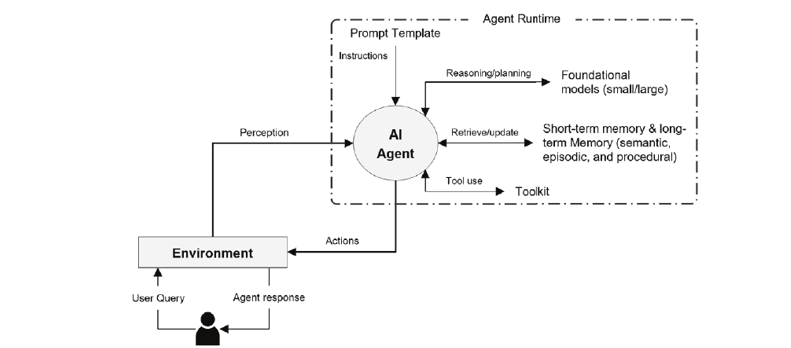
\includegraphics[width=0.86\textwidth]{fig_agent_arch.png}
\caption{AI agent architecture (adapted from \cite{ref1}).}\label{fig:agent}
\end{figure}

The main components are explained below:
\begin{itemize}[leftmargin=*]
  \item \textbf{Prompt Template:} Provides instructions that guide the agent in understanding the request and deciding which actions to perform.
  \item \textbf{Foundational Model:} Processes user queries, supports reasoning and generates suitable responses.
  \item \textbf{Short-term Memory:} Stores temporary information related to the current interaction, such as the driver's location and parking search results.
  \item \textbf{Long-term Memory:} Stores user preferences, previous experiences and information that can be useful in future interactions.
  \item \textbf{Toolkit:} Connects the agent to external services such as parking APIs, GPS, mapping services and payment systems.
  \item \textbf{Environment:} Represents the surroundings with which the agent interacts to receive information and perform actions.
\end{itemize}

For example, when a driver asks for a parking spot, the agent checks the current location, considers the driver's preferences, searches available parking options and provides a suitable recommendation.

\subsection{Sequence of a Parking Request}
Figure~\ref{fig:seq} presents the sequence of interactions between the driver, AI agent, model, memory components and external tools during a parking request.

\begin{figure}[htbp]
\centering
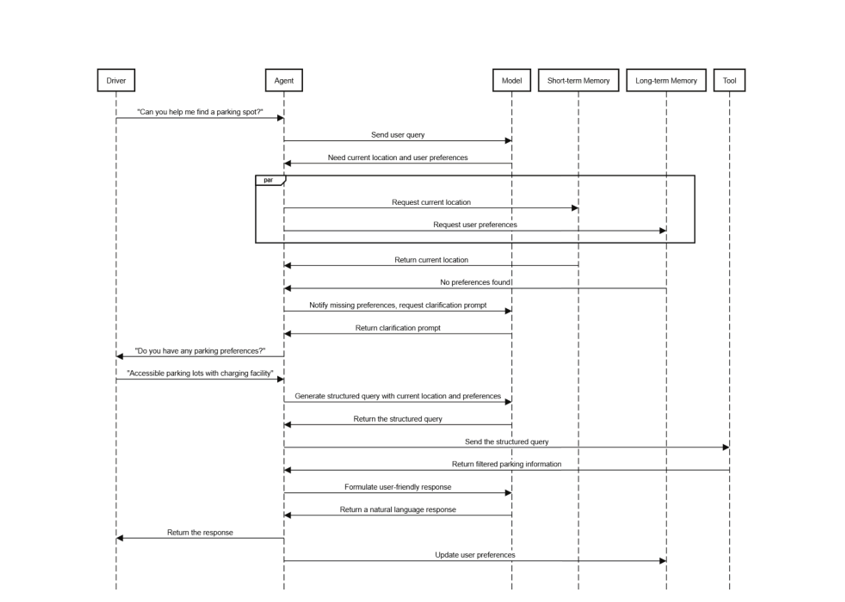
\includegraphics[width=0.82\textwidth]{fig_sequence.png}
\caption{Sequence diagram of a parking request (adapted from \cite{ref1}).}\label{fig:seq}
\end{figure}

The process follows these steps:
\begin{enumerate}[leftmargin=*]
  \item The driver requests assistance in finding a parking spot.
  \item The agent sends the query to the foundational model for processing.
  \item The agent retrieves the current location from short-term memory and checks long-term memory for stored preferences.
  \item If preferences are unavailable, the agent asks the driver for clarification.
  \item The driver provides preferences, such as accessible parking and EV charging facilities.
  \item The agent combines the current location and preferences to prepare a structured search query.
  \item The query is sent to an external parking API or toolkit.
  \item The toolkit returns parking information matching the search criteria.
  \item The model processes the results and generates a natural-language response.
  \item The agent presents the recommendation to the driver and updates long-term memory with the new preferences.
\end{enumerate}

This sequence demonstrates how an AI agent combines user input, memory, reasoning and external tools to complete a task. The agent may use step-by-step reasoning to identify the required information, filter available parking spaces and rank the results according to the driver's preferences. This structured process can help improve the relevance and reliability of recommendations.

% ----------------------------- CHAPTER 5 ---------------------------
\chapter{APPLICATIONS}
Agentic AI can be used in different fields to perform tasks step by step. It uses AI agents, memory and external tools to understand user needs and provide suitable solutions. Some important applications are explained below.

\section{Smart Urban Parking}
Finding a parking space in busy cities is often difficult and takes a lot of time. Normal parking apps help users find parking or make payments, but they may not manage the complete process. Agentic AI can help users find a suitable parking space, navigate to it, enter the parking area and leave easily. It can also consider user preferences, such as parking cost, accessibility and EV charging facilities.

\section{EV Charging and In-Vehicle Assistants}
Agentic AI can be used in vehicle assistants to help drivers find parking spaces with EV charging facilities. It can check the availability of charging points, guide drivers to the location and provide updates about charging. It can also help people with disabilities find accessible parking spaces near entrances.

\section{Smart Mobility and Smart Cities}
Agentic AI can help improve transportation in smart cities. It can use traffic updates, location information and parking availability to help people travel more easily. It can also reduce the time spent searching for parking and help reduce traffic congestion. Different agents can work together to provide services such as navigation, parking and EV charging.

\section{Other Industry Domains}
Agentic AI can also be used in areas such as data management, networking, retail and marketing. In these fields, different agents can handle different tasks and work together to achieve a common goal. This reduces manual work and makes complex processes easier to manage. The performance of these systems depends on the AI model, instructions and tools used.

Multiagent collaboration for autonomous task execution can be applied in various domains where complex tasks require multiple steps, specialized capabilities, communication, and coordination among agents. Different agents can perform specific responsibilities, exchange information, verify results, and contribute toward a common objective.

\section{Software Development}
Multiagent collaboration can be used in software development to divide development tasks among specialized agents. A planner agent can organize the task, while coder agents can generate code. Testing agents can check the developed code, while review agents can identify errors or suggest improvements. Communication between these agents supports collaborative development, code review, debugging, and verification.

\section{Workflow Automation}
Multiagent systems can automate complex workflows by dividing a business task into smaller subtasks. A coordinator agent can identify the required steps and assign them to specialized agents. The agents perform their respective tasks, share the results, and the coordinator combines the outputs. This reduces the need for continuous human intervention in multi-step workflows.

\section{Data Analysis}
Multiagent collaboration can support data analysis by assigning different stages of the analysis process to different agents. One agent can gather or prepare data, another can perform analysis, while another can check or summarize the results. The agents can exchange information during the process to improve the accuracy and organization of the final output.

\section{Autonomous Task Execution}
Multiagent collaboration can be used for complex autonomous tasks that require continuous planning, decision-making, and coordination. Different agents can handle specific parts of the task based on their capabilities. They can communicate, share knowledge, provide feedback, and adjust their actions according to changes during execution. This supports scalable automation with reduced human intervention.

% ----------------------------- CHAPTER 6 ---------------------------
\chapter{ADVANTAGES AND LIMITATIONS}
\section{Advantages}
\begin{itemize}[leftmargin=*]
  \item \textbf{Complete parking journey:} the architecture covers search, guidance, access, micro-routing, on-spot services and departure, whereas existing parking apps address only parts of the journey.
  \item \textbf{Context-aware personalisation:} memory and the personalised cloud profile let the system apply hard and soft constraints and learn from past interactions and post-trip feedback.
  \item \textbf{Modular and extensible design:} each specialised agent has a clearly defined role and can be developed, improved or replaced without redesigning the whole system.
  \item \textbf{Flexible collaboration:} augmentative, integrative and debative cooperation, together with cueing and handoff, improve efficiency, expertise and reliability.
  \item \textbf{Reliable recommendations:} input and output guardrails and Chain-of-Thought prompting check constraints and plausibility, and the ethics module addresses bias and privacy.
\end{itemize}
\section{Limitations}
\begin{itemize}[leftmargin=*]
  \item \textbf{Partial implementation:} Only two agents are implemented and tested. The remaining five agents are still conceptual.
  \item \textbf{Limited evaluation:} The system is tested using only a few performance measures. Human feedback and comparison with other systems are missing.
  \item \textbf{Inconsistent responses:} AI may give different answers to the same question, especially when the request is unclear.
  \item \textbf{Hardware and data dependency:} The system depends on external APIs and internet data. Its performance may vary depending on the hardware used.
  \item \textbf{Limited model testing:} Only four OpenAI models are tested, and the system's cooperation methods need further development.
  \item \textbf{Privacy and infrastructure:} The system requires smart parking facilities and user location data, so proper infrastructure and privacy protection are necessary.
\end{itemize}

% ----------------------------- CHAPTER 7 ---------------------------
\chapter{CONCLUSION}
This seminar studied the research paper ``Agentic AI Systems: Architecture and Evaluation Using a Frictionless Parking Scenario''~\cite{ref1}. The paper proposes an AI-based parking system with seven specialised agents that help drivers throughout the parking journey, from finding a parking space to leaving the parking area.

The paper explains how different agents can work together using cooperation methods such as augmentative, integrative and debative cooperation. It also describes two ways for agents to interact: cueing and handoff. However, existing AI frameworks do not fully support these methods.

The researchers implemented and tested only two agents: the Interaction Agent and the Informative Search Agent. The results showed that smaller AI models with shorter responses provide faster and more consistent results. Clear prompts and simple tasks also help improve system performance.

In the future, the system can be improved by testing more AI models, adding long-term memory and implementing the remaining five agents. Overall, Agentic AI has the potential to make parking easier, save time and improve smart mobility services.

% ----------------------------- REFERENCES --------------------------
\renewcommand{\bibname}{References}
\begin{singlespacing}
\begin{thebibliography}{99}
\addcontentsline{toc}{chapter}{REFERENCES}
\bibitem{ref1} A. Khamis, ``Agentic AI Systems: Architecture and Evaluation Using a Frictionless Parking Scenario,'' \emph{IEEE Access}, vol. 13, pp. 126052--126069, 2025.
\bibitem{ref2} D. B. Acharya, K. Kuppan, and B. Divya, ``Agentic AI: Autonomous Intelligence for Complex Goals---A Comprehensive Survey,'' \emph{IEEE Access}, vol. 13, pp. 18912--18936, 2025.
\bibitem{ref3} Y. Xiao, G. Shi, and P. Zhang, ``Towards Agentic AI Networking in 6G: A Generative Foundation Model-as-Agent Approach,'' arXiv preprint arXiv:2503.15764, 2025.
\bibitem{ref4} L. N. Mishra and B. Senapati, ``Retail Resilience Engine: An Agentic AI Framework for Building Reliable Retail Systems With Test-Driven Development Approach,'' \emph{IEEE Access}, vol. 13, pp. 50226--50243, 2025.
\bibitem{ref5} N. Kshetri, ``From Predictive and Generative to Agentic AI: Shaping the Future of Marketing Operations and Strategies,'' \emph{Computer}, vol. 58, no. 4, pp. 121--129, 2025.
\bibitem{ref6} A. Khamis, ``Agentic AI Systems: Architecture and Evaluation Using a Frictionless Parking Scenario,'' \emph{IEEE Access}, vol. 13, pp. 126052--126069, 2025.
\bibitem{ref7} E. Miehling \emph{et al.}, ``Agentic AI Needs a Systems Theory,'' arXiv preprint arXiv:2503.00237, 2025.
\bibitem{ref8} H. Derouiche, Z. Brahmi, and H. Mazeni, ``Agentic AI Frameworks: Architectures, Protocols, and Design Challenges,'' arXiv preprint arXiv:2508.10146, 2025.
\end{thebibliography}
\end{singlespacing}

\end{document}
